%!TEX root = ../hall.tex
% Тип документа
\documentclass[a4paper,12pt]{extarticle}

% Шрифты, кодировки, символьные таблицы, переносы
% \usepackage{cmap}
% \usepackage[T2A]{fontenc}
\usepackage[utf8]{inputenc}
\usepackage[russian]{babel}
% Это пакет -- хитрый пакет, он нужен но не нужен
\usepackage[mode=buildnew]{standalone}

\usepackage
	{
		% Дополнения Американского математического общества (AMS)
		amssymb,
		amsfonts,
		amsmath,
		amsthm,
		% Пакет для физических текстов
		physics,
		% misccorr,
		% 
		% Графики и рисунки
		wrapfig,
		graphicx,
		subcaption,
		float,
		tikz,
		tikz-3dplot,
		caption,
		csvsimple,
		color,
		booktabs,
		geometry,
		% 
		% Таблицы, списки
		makecell,
		multirow,
		indentfirst,
		%
		% Интегралы и прочие обозначения
		ulem,
		esint,
		esdiff,
		% 
		% Колонтитулы
		fancyhdr,
	}  
\usepackage{pgfplots,pgfplotstable,booktabs,colortbl}
\usepackage{xcolor}
\usepackage{hyperref}
\usepackage{pythontex}
 % Цвета для гиперссылок
\definecolor{linkcolor}{HTML}{000000} % цвет ссылок
\definecolor{urlcolor}{HTML}{799B03} % цвет гиперссылок
 
\hypersetup{pdfstartview=FitH,linkcolor=linkcolor,urlcolor=urlcolor, colorlinks=true}
\hypersetup{pageanchor=false}
% Увеличенный межстрочный интервал, французские пробелы
\linespread{1.3} 
\frenchspacing 

 
% \usetikzlibrary
% 	{
% 		decorations.pathreplacing,
% 		decorations.pathmorphing,
% 		patterns,
% 		calc,
% 		scopes,
% 		arrows,
% 		fadings,
% 		through,
% 		shapes.misc,
% 		arrows.meta,
% 		3d,
% 		quotes,
% 		angles,
% 		babel
% 	}
% Среднее <#1>
\newcommand{\mean}[1]{\langle#1\rangle}

\begin{pycode}
##
def frexp10(decimal):
	parts = ('%e' % decimal).split('e')
	return float(parts[0]), int(parts[1])
##
\end{pycode}



% Функция для тех, кто использует pythontex. Представляет любое вещественное число в стандартном виде.
\newcommand{\frexp}[1]{
		\pyc{#10=frexp10(#1)} 
			\py{ round(#10[0],2)} 
				\cdot 10^{\py{#10[1]}} }

% const прямым шрифтом
\newcommand\ct[1]{\text{\rmfamily\upshape #1}}
\newcommand*{\const}{\ct{const}}
\usepackage{array}
\usepackage{pstool}

\geometry		
	{
		left			=	2cm,
		right 			=	2cm,
		top 			=	2.5cm,
		bottom 			=	2.5cm,
		bindingoffset	=	0cm
	}

%%%%%%%%%%%%%%%%%%%%%%%%%%%%%%%%%%%%%%%%%%%%%%%%%%%%%%%%%%%%%%%%%%%%%%%%%%%%%%%
	%применим колонтитул к стилю страницы
\pagestyle{fancy} 
	%очистим "шапку" страницы
% \fancyhead{} 
	%слева сверху на четных и справа на нечетных
\fancyhead[R]{}%\labauthors 
	%справа сверху на четных и слева на нечетных
% \fancyhead[L]{Отчёт по лабораторной работе №\labnumber}
\fancyhead[L]{\labtheme} 
	%очистим "подвал" страницы
% \fancyfoot{} 
	% номер страницы в нижнем колинтуле в центре
\fancyfoot[C]{\thepage} 

%%%%%%%%%%%%%%%%%%%%%%%%%%%%%%%%%%%%%%%%%%%%%%%%%%%%%%%%%%%%%%%%%%%%%%%%%%%%%%%

\renewcommand{\contentsname}{Оглавление}
\usepackage{tocloft}
\usepackage{secdot}
\sectiondot{subsection}


\begin{pycode}
##
from main import *
##
\end{pycode}

\renewcommand{\phi}{\varphi}

\begin{document}

\def\labauthors{Виноградов И.Д., Шиков А.П.}
\def\labgroup{430}
\def\labnumber{1}
\def\labtheme{Измерение ширины запрещенной зоны}
\def\department{}
\begin{titlepage}

\begin{center}

{\small\textsc{Нижегородский государственный университет имени Н.\,И. Лобачевского}}
\vskip 1pt \hrule \vskip 3pt
{\small\textsc{Радиофизический факультет. Кафедра Радиотехники.}}

\vfill

{\Large Отчет по лабораторной работе №\labnumber\vskip 12pt\bfseries \labtheme}
	
\end{center}

\vfill
	
\begin{flushright}
	{Выполнили студенты \labgroup\ группы\\ \labauthors}%\vskip 12pt Принял:\\ Менсов С.\,Н.}
\end{flushright}
	
\vfill
	
\begin{center}
	Нижний Новгород, \the\year
\end{center}

\end{titlepage}



% \tableofcontents

\newpage
\section*{Введение}
Ширина запрещенной зоны является одной из важнейших характеристик полупроводниковых материалов. Она может быть найдена
по результатам измерений электропроводности или постоянной Холла в зависимости от температуры, а также из спектрального 
распределения коэффициента оптического поглощения или фототока полупроводника. В настоящей работе студентам предлагается
определить величину ширины запрещенной зоны полупроводникового материала по результатам измерения температурной зависимости 
электропроводности. 
\begin{wrapfigure}{l}{0.5\linewidth}
	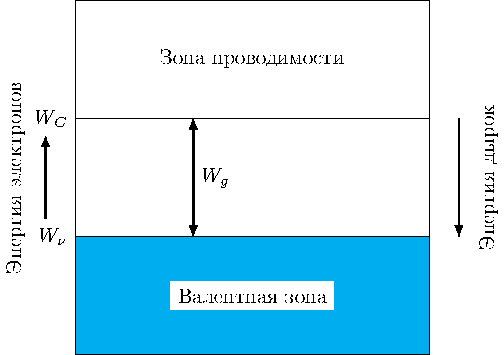
\includegraphics[width = \linewidth]{img/cond.pdf}
	\caption{Энергитический спектр электрона в кристалле. $W_c,W_{\nu}$ - соответственно, энергии дна зоны проводимости и потолка валентной зоны, $W_g$ - ширина запрещенной зоны.}
	\label{fig:cond}
\end{wrapfigure}
В изолированном атоме электроны находятся в стационарных состояниях, каждому из которых соответствует строго
определенное значение энергии. Таким образом, энергетический спектр электронных состояний в атоме является дискретным. В
кристаллическом твердом теле из-за возмущений, вносимых другими атомами, уровни энергии расщепляются – образуются
области или зоны разрешенных значений энергии, между которыми находятся запрещенные зоны. Для глубоких уровней
расщепление невелико, т.к. находящиеся на них электроны экранируются верхними оболочками и практически не
взаимодействуют с соседними атомами. 

\section{Концентрация носителей заряда в полупроводнике}
Вычисление концентрации подвижных и связанных носителей заряда в полупроводнике составляет задачу статистики электронов.
Решение этой задачи, с одной стороны, позволяет объяснить экспериментальные результаты, по которым, в свою очередь,
становится возможным определение ряда важных характеристик полупроводника (ширины запрещенной зоны, энергия ионизации примеси).
Задача вычисления концентрации носителей заряда распадается на две:  1) определение числа возможных квантовых состояний
электронов в разрешенных зонах в твердом теле и 2) выяснение фактического распределения электронов по этим квантовым
состояниям. Рассмотрим последовательно решение каждой из подзадач.

Число состояний в любой зоне кристалла равно общему числу мест на уровнях изолированных атомов, образовавших кристалл,
т.е. числу атомов $N_0$, умноженному на кратность вырождения $\nu$ атомного уровня, образовавшего данную зону:

\begin{equation}
	\int \limits_{W_1}^{W_2} N(W) dW  =\nu N_0 
	\label{eq:2.1}
\end{equation} 

где $N(W)dW$ - число  квантовых состояний в интервале энергий от $W$ до $W+dW$ в единице объёма полупроводника, а $N(W)$
-  плотность квантовых состояний. $W_1,W_2$ - энергии нижнего и верхнего края зоны, соответственно. 

Выражение для плотности квантовых состояний у дна зоны проводимости:
\begin{equation}
	N_{c}(W)=\frac{d Z}{d W}=4 \pi\left[\frac{2 m_{n}^{*}}{(2 \pi \hbar)^{2}}\right]^{3 / 2} \sqrt{W-W_{C}}
	\label{eq:2.7}
\end{equation} 

Статистика электронов подчиняется распределение Ферми-Дирака:   
\begin{equation}
	f(W) = \frac{1}{\exp(\frac{W-W_F}{k_B T})+1}
	\label{eq:2.8}
\end{equation}
которое даёт вероятность того, что в тепловом равновесии состояние с энергией $W$ занято электроном. Здесь $k_B$ –
постоянная Больцмана, $T$ – абсолютная температура, $W_F$ – энергия (уровень) Ферми – максимальная энергия электронов при
абсолютном нуле. Для температуры, отличной от нуля, функция $f(W)$ в точке $W = W_F$ имеет перегиб.

Выражения для концентрации электронов и дырок в совокупности с принципом электронейтральности
полупроводника ( в однородном полупроводнике не может быть существенных нескомпенсированных объемных зарядов ни в
равновесном состоянии, ни при наличии тока ) позволяют сделать выводы о положении уровня Ферми в полупроводнике.
Рассмотрим собственный полупроводник, для которого влияние примесных атомов не существенно. Свободные носители заряда в
этом случае возникают только за счет разрыва валентных связей. Поэтому в собственном полупроводнике концентрация дырок p
равна концентрации электронов $ n: n = p \equiv n_i$. Это условие электронейтральности собственного полупроводника.

Уровень Ферми $W_F$ собственного полупроводника при абсолютном нуле температуры лежит в центре запрещенной зоны и,
вообще говоря, смещается при возрастании температуры. Этот случай показан на рис.\ref{fig:2.1}(a), где слева направо схематически
приведены простейшая зонная диаграмма, плотность состояний $N(W)$, распределение Ферми $f (W)$ и концентрация носителей
заряда.

\begin{figure}[h!]
	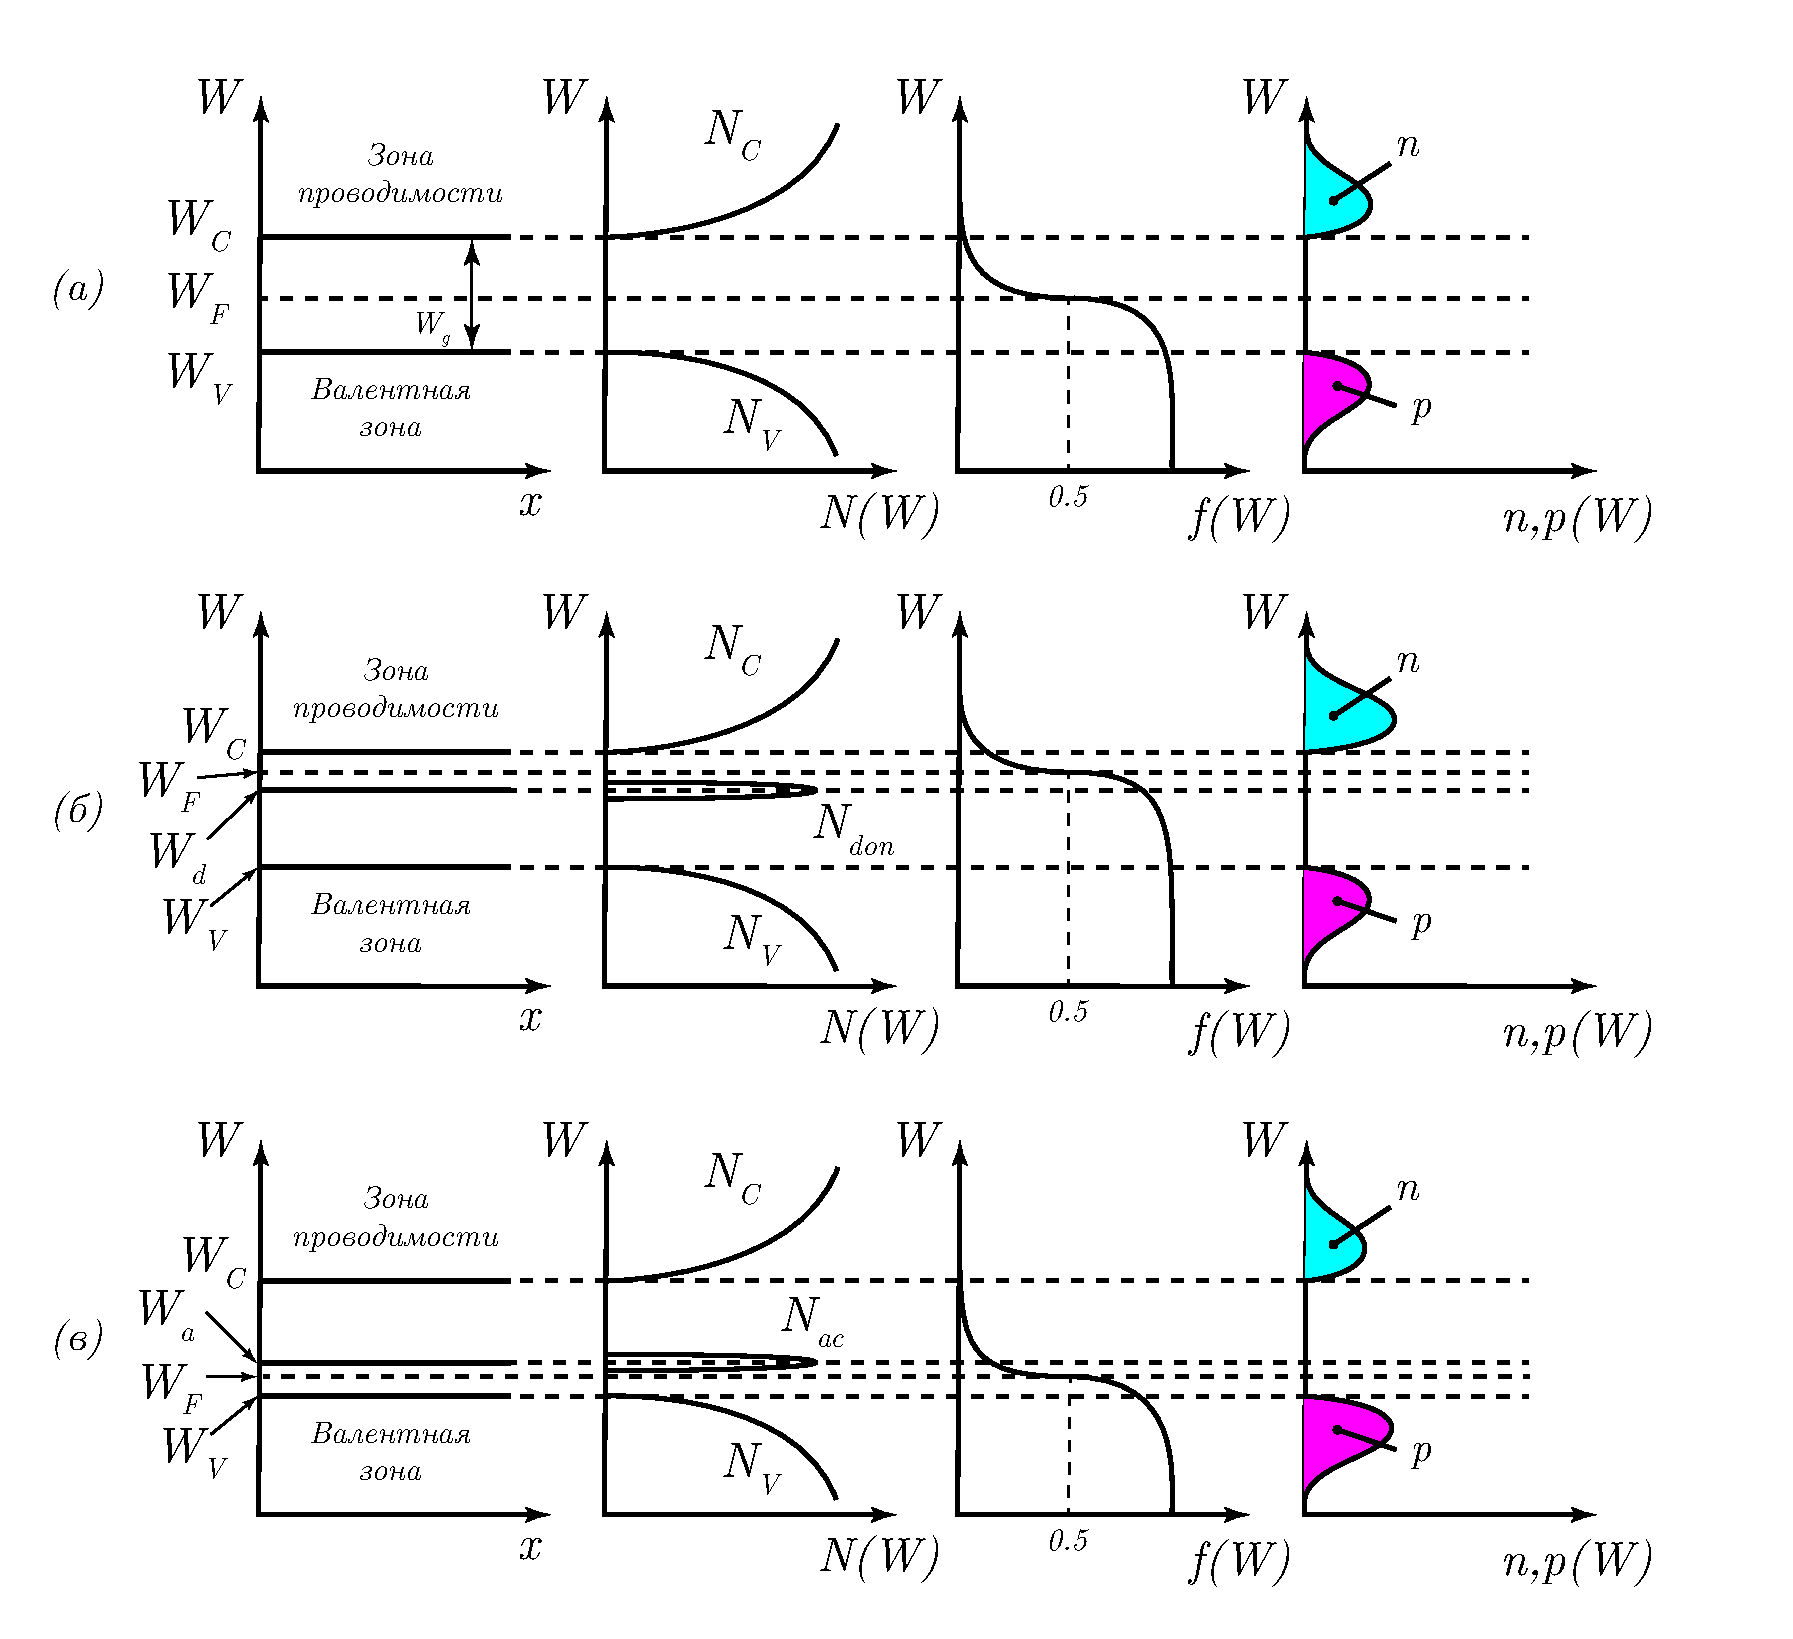
\includegraphics[width = \linewidth]{img/22}
	\caption{Графическое изображение решения уравнения электронейтральности для собственного полупроводника(а), для примесного полупроводника, легированного донорной (б) и акцепторной (в) примесью}
	\label{fig:2.1}
\end{figure}


\section{Подвижность носителей заряда в полупроводнике}
В реальной кристаллической структуре всегда присутствуют дефекты: тепловые колебания атомов решётки, примеси и т.д.
Поэтому при воздействии внешнего электрического поля частица движется ускоренно лишь на небольшом участке пути, а затем
испытывает рассеяние (взаимодействие с дефектами кристалла), изменяя свой импульс и ( в случае неупругого
взаимодействия) энергию, теряет направленную скорость, после чего процесс разгона начинается заново (рис. \ref{fig:3.1}). В слабых
электрических полях ($\leq 10^3$ В/см) средняя скорость направленного движения носителей заряда (дрейфовая скорость)
пропорциональна напряжённости электрического поля:$\nu = \mu E$. Коэффициент пропорциональности между скоростью и полем $\mu$
называется подвижностью носителей заряда. Эта величина численно равна средней скорости направленного движения частиц в
электрическом поле с напряженностью 1 В/м. 

Рассеяние носителей заряда на нейтральных атомах примеси и нейтральных дефектах является слабым. Однако, при низких
температурах, когда примеси еще практически не ионизованы, а тепловые колебания отсутствуют, этот механизм играет
существенную роль. Для того, чтобы электрон изменил направление своего движения в результате взаимодействия с
нейтральной примесью или дефектом, необходимо, чтобы траектория электрона проходила через место расположения дефекта
либо через примыкающую к нему область решетки, в которой им вызваны искажения. Рассеяние на нейтральных примесях не
зависит от температуры, а подвижность, обусловленная этим рассеянием, постоянна и зависит только от концентрации
рассеивающих центров.

\begin{wrapfigure}{l}{0.3\linewidth}
	\centering
	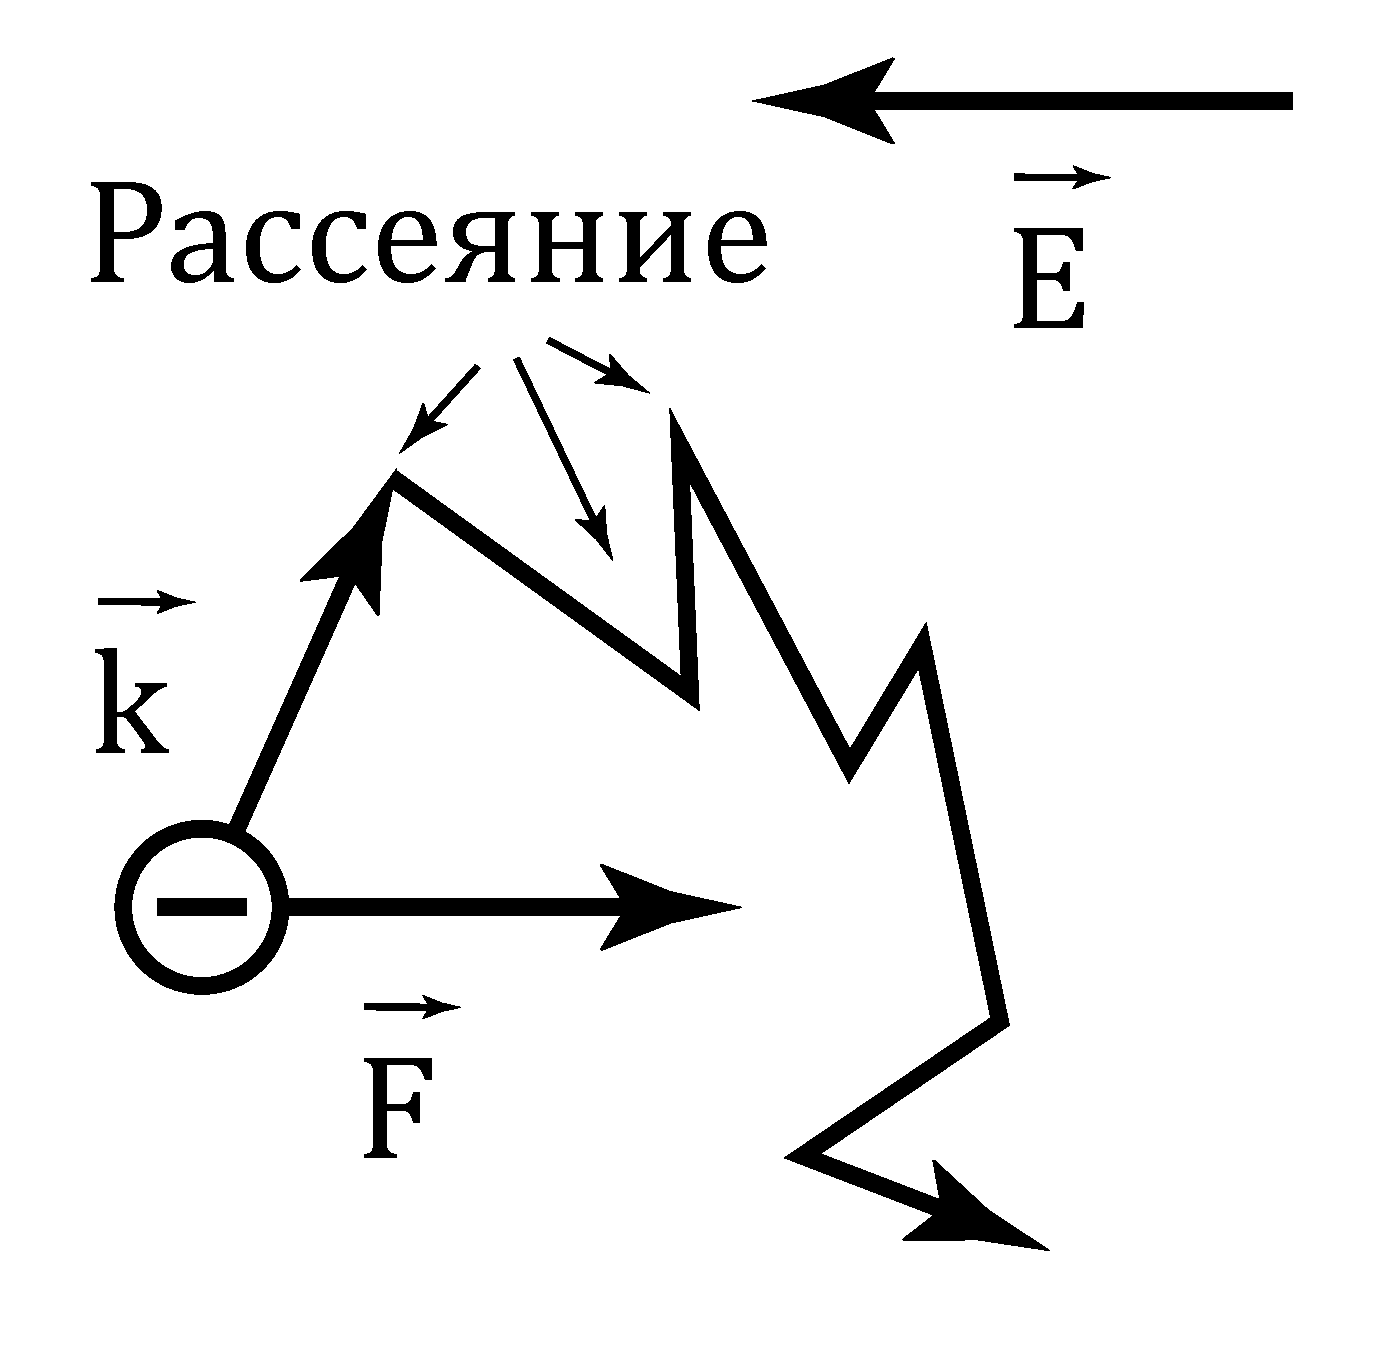
\includegraphics[width = .9\linewidth]{img/31}
	\caption{Схематическое изображение движения электрона в полупроводнике под действием электрического поля.}
	\label{fig:3.1}
\end{wrapfigure}

Электрическое поле ионизованного примесного атома распространяется на много периодов кристаллической решетки, и
электрон, проходя на значительном расстоянии от иона, изменит под действием его поля направление своего движения. Пусть
рассеяние в полупроводнике происходит только на ионах примеси, а тепловые колебания и нейтральные центры рассеяния
отсутствуют. Тогда, как показывают расчеты, подвижность зависит от температуры как $T^{3/2}$, т.е. увеличивается. Этот
результат легко понять, если учесть, что с ростом температуры увеличивается средняя скорость хаотического движения
электронов, а быстрые электроны слабее отклоняются статическим полем ионов. Этот механизм рассеяния играет основную роль
при температурах, когда уже имеется большая концентрация ионизированных примесей, но тепловые колебания еще мало влияют
на рассеяние. 

\section{Температурная зависимость проводимости}
Плотность тока, создаваемого всеми свободными электронами, равна:
\begin{equation}
	j=e n \mu_{n} E=\sigma_{n} E
	\label{eq:4.1}
\end{equation}
где n – концентрация электронов, $\sigma_n = e n \mu_n$ – удельная проводимость полупроводника, обусловленная электронами.
Если имеется два типа носителей в полупроводнике – электроны и дырки,
то проводимость равна:
\begin{equation}
	\sigma=e\left(n \mu_{n}+p \mu_{p}\right)
	\label{eq:4.2}
\end{equation}
Для определения температурной зависимости проводимости необходимо перемножить зависимости концентрации и подвижности носителей заряда от
температуры. При низких температурах и неполной ионизации примесей концентрация зависит от обратной температуры по
экспоненциальному закону, а подвижность – по степенному, т.е. температурная зависимость концентрации определяет
температурную зависимость проводимости:
\begin{equation}
	\sigma=\sigma_{d} e^{\left(-\Delta W_{d} / 2 k_{B} T\right)}
	\label{eq:4.3}
\end{equation}
Здесь $\sigma_d$ содержит степенную зависимость подвижности и эффективной плотности состояний от температуры.

В области истощения примесей концентрация не зависит от температуры, поэтому в этой области температурная зависимость проводимости определяется
степенной зависимостью подвижности от температуры. И, наконец, при больших температурах зависимость проводимости от
обратной температуры экспоненциальна, т.к. $\mu \approx T^{3/2}$, а  $N_c \approx T^{3/2}$:
 \begin{equation}
	\sigma=\sigma_{c} e^{\left(-W_{g} / 2 k_{B} T\right)}
	 \label{eq:4.4}
 \end{equation}
 \begin{figure}[h!]
	\centering
	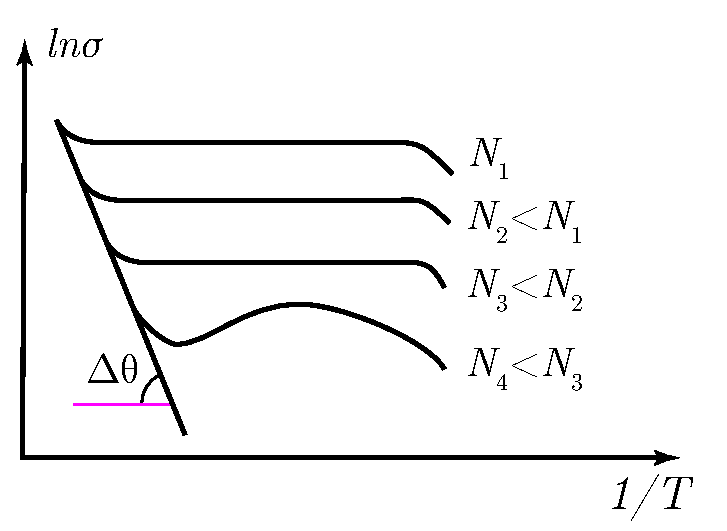
\includegraphics[width = .5\linewidth]{img/41}
	\caption{Качественный вид зависимости удельной проводимости полупроводника от температуры для различных уровней легирования (N-концентрация легирующей примеси)}
	\label{fig:4.1}
\end{figure}
На рис. \ref{fig:4.1} показана зависимость $\ln(\sigma)$ от обратной температуры при различных уровнях легирования полупроводника. По
экспериментально измеренным зависимостям $\sigma(T)$ , аналогичным рис.\ref{fig:4.1}, можно определить ширину запрещенной зоны и
энергию активации примесей. 



\newpage
\section{Методика измерений}

\begin{figure}[h!]
	\centering
	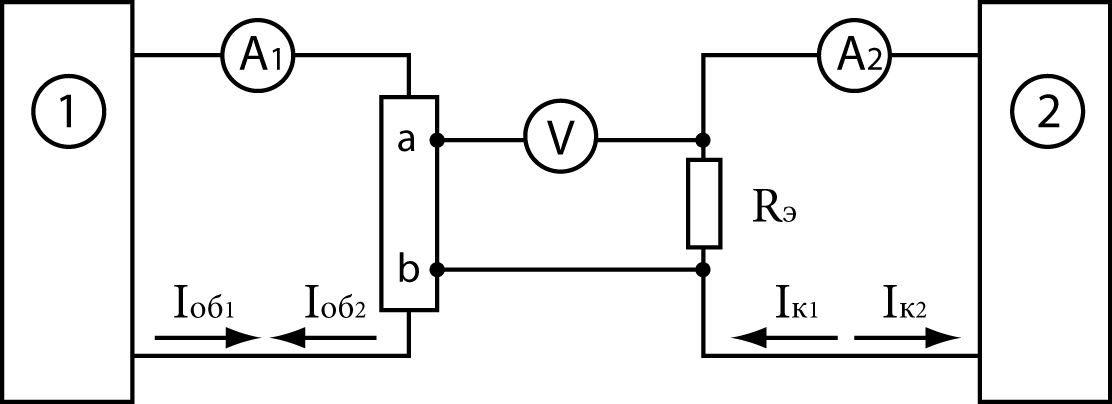
\includegraphics[width = .9\linewidth]{img/scheme.jpg}
	\caption{Электрическая схема для измерений удельной электропроводности методом компенсации}
	\label{fig:5.1}
\end{figure}

Регулируемый источник тока (1) задаёт ток образца $I_\text{об}$, измеряемый амперметром $A1$. Регулируемый источник тока
(2) задаёт ток компенсации $I_\text{к}$ через эталонный резистор $R_\text{э}$, величина этого тока измеряется
амперметром $А2$. Напряжение $U_{ab}$ между зондовыми электродами a и b сравнивается с напряжением компенсации $U_k$ на
эталонном резисторе $R_\text{э}$ при помощи индикатора компенсации V.

При проведении измерений нужно установить ток образца, затем, изменяя ток компенсации, добиться нулевых показаний
индикатора компенсации V. В этом случае напряжение $U_k$ на эталонном резисторе $R_\text{э}$ будет равно напряжению $U_{ab}$:
\begin{equation}
	U_{ab}=U_{k}=I_{k} R_{\text{э}} 
	\label{eq:5.1}
\end{equation}

В реальной ситуации между зондовыми электродами будут паразитные потенциалы, связанные, во-первых, с влиянием
переходного сопротивления на контактах «образец – подводящие провода», во-вторых, появлением термоЭДС на контактах
полупроводника с металлом при нагреве образца. Для того чтобы устранить влияние этих потенциалов, измерение тока
компенсации производится дважды. Получив первый отсчёт $I_{k1}$, изменяем направление тока через образец и через
эталонный резистор, опять добиваемся равенства напряжений $U_k$ и $U_{ab}$, снимаем второй отсчёт $I_{k2}$. Обратите
внимание, что полярность разности потенциалов между электродами a и b, вызванная протеканием тока через образец, как и
напряжение на $R_\text{э}$, сменились на противоположные, а паразитные потенциалы, зависящие от свойств контактов, и
термоЭДС, зависящая от температуры образца, остались прежние. Таким образом, среднеарифметическое значение 

$$I_k=\frac{I_{k1}+I_{k2}}{2}$$

будет содержать информацию только о полезной составляющей напряжения $U_{ab}$.

Величину падения напряжения $U_k$ легко подсчитать:
$$U_{k}=I_{k} R_{\text{э}}$$

Величину сопротивления участка образца расположенного между зондовыми электродами a и b ($R_{\text{об}}$) можно определить из равенства:
$$R_{\text{об}}=\frac{U_{k}}{I_{\text{об}}}=\frac{I_{k} R_{\text{э}}}{I_{\text{об}}}$$
Зная размеры образца: a - ширина (см), d - толщина (см), l - расстояние между электродами a и b (см), можно рассчитать удельное сопротивление образца:
$$\rho=\frac{d a}{l} R_{\text{об}} (\text{Oм} \text{ cм})$$

или обратную величину - удельную электропроводность: 
$$\sigma=1 / \rho\left(\text{Oм}^{-1} \text{cм}^{-1}\right)$$

\section{Схема экспериментальной установки}

\begin{figure}[h!]
	\centering
	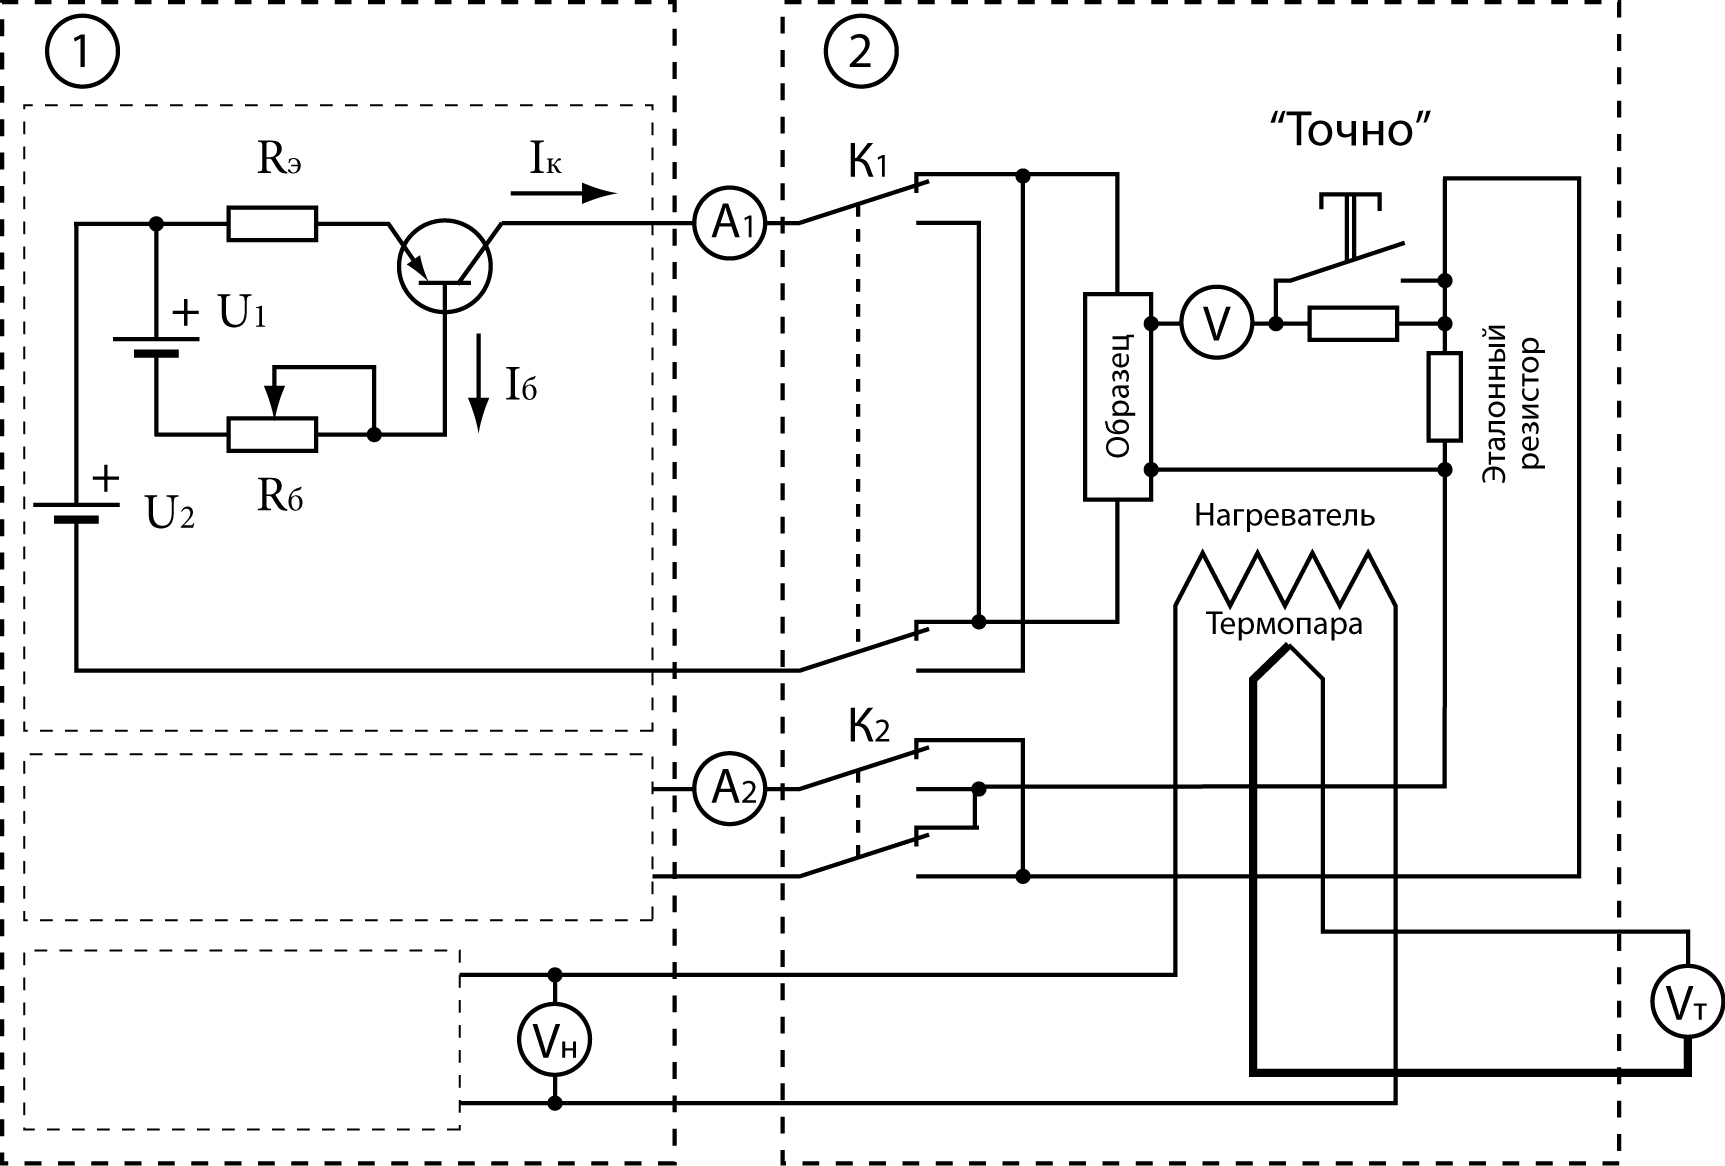
\includegraphics[width = .8\linewidth]{img/scheme-2.jpg}
	\caption{Схема установки}
	\label{fig:6.2}
\end{figure}

Блок питания (1) содержит в себе два регулируемых стабилизатора тока (для образца и эталонного резистора) и регулируемый
источник питания нагревателя образца, напряжение на выходе которого контролируется вольтметром $V_\text{н}$. На верхней
крышке измерительного блока (2) находится трубчатый керамический нагреватель, в котором размещён исследуемый образец и
термопара для измерения температуры. Нагреватель с образцом и термопарой закрыты защитным цилиндром. В корпусе
измерительного блока (2) располагается эталонный резистор Rэ, переключатели направления тока образца и компенсации К1 и
К2, индикатор компенсации V с переключателем чувствительности «Точно». Измерение токов образца и компенсации
производится миллиамперметрами А1 и А2 для измерения ЭДС термопары используется милливольтметр Vт, показания которого
пересчитываются в температуру по градуировочному графику (рис. \ref{fig:6.3}).

\begin{figure}[h!]
	\centering
	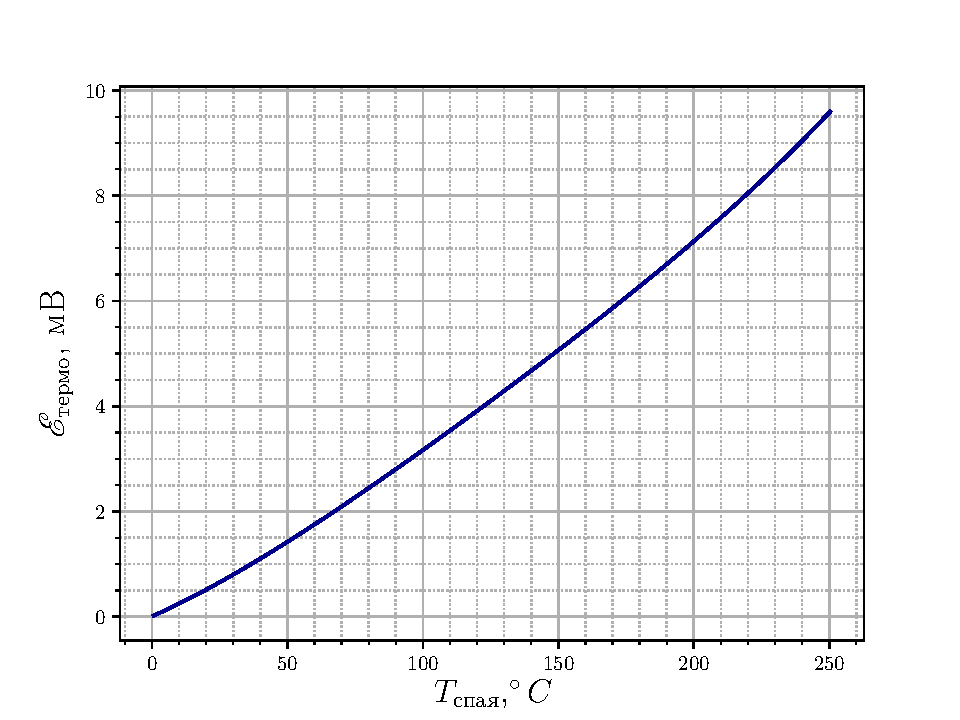
\includegraphics[width = .9\linewidth]{img/grad.pdf}
	\caption{График соответствия ЭДС термопары и температуры спая}
	\label{fig:6.3}
\end{figure}

\newpage
\section*{Эксперимент}
\textbf{Оборудование}
\begin{enumerate}
	\item $R{\text{э}} = 10$ Ом.
	\item Образец $l = 7$ см, $d=1.4$ см, $a = 4$ см $x = 20$ см.
\end{enumerate}

Произвели измерение электропроводности образца при комнатной температуре. Установив ток образца 5-10 мА
добились нулевого отклонения индикатора. Аналогичное сделали, сменив направление тока.

Такие же измерения провели при различных температурах. Сняли температурную зависимость тока компенсации (для двух направлений тока при каждом
значении температуры $I_{k1},I_{k2}$).

Далее взяли среднее значение тока:
$$I_k=\frac{I_{k1}+I_{k2}}{2}$$

Рассчитали проводимость для каждой снятой точки по формуле:

$$\sigma = \frac{l}{ad} \frac{I_{\text{об}}}{ I_k ~ R_{\text{э}}}$$


\subsection*{Обработка результатов измерений}
Построили график (см рис. \ref{fig:exp.1} ) полученной зависимости $\ln~\sigma(\frac{10^3}{T})$ (Т – абсолютная температура в градусах К).

\begin{figure}[h!]
	\centering
	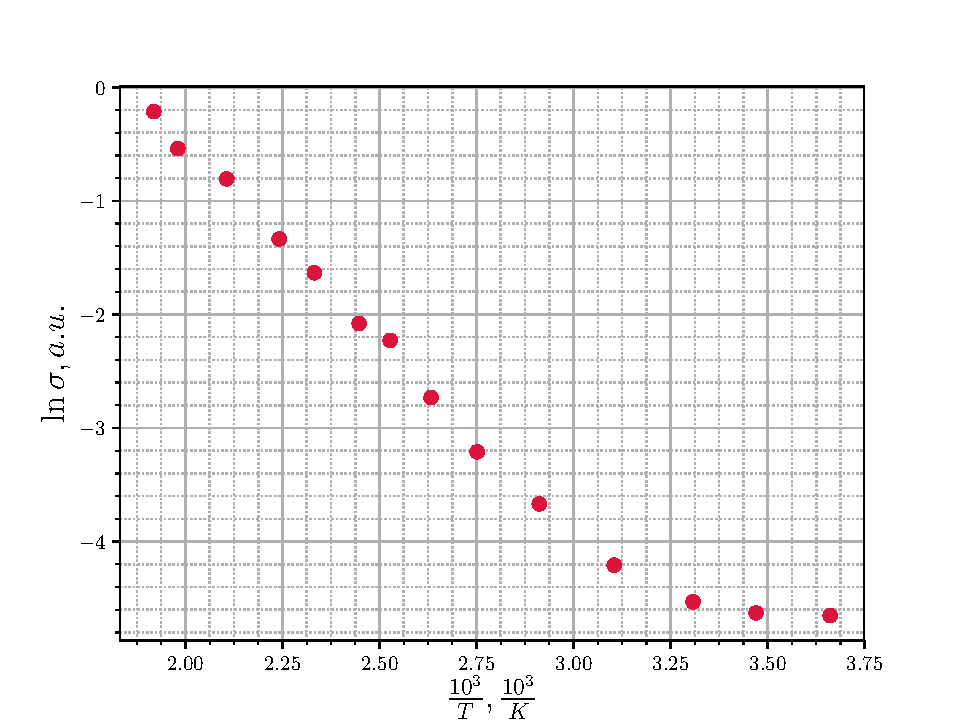
\includegraphics[width = .8\linewidth]{fig/lns}
	\caption{}
	\label{fig:exp.1}
\end{figure}

Прологарифмировали выражение \eqref{eq:4.4} и нашли связь между угловым коэффициентом наклона кривой
$\ln\sigma(\frac{10^3}{T})$ и величиной $W_g$:

$$ \ln(\sigma) = \underbrace{\ln(\sigma_C)}_{const} - W_g /2 k_B T $$
$$ W_g = -1000 \cdot \tan(\theta) \cdot 2 k_B $$
где $\tan(\theta)$ - тангенс угла наклона графика 
$\ln\sigma(\frac{1}{T})$, 
$k_B \approx 8.62 \cdot 10^{-5}$ эВ/К -
постоянная Больцмана.

\begin{figure}[h!]
	\centering
	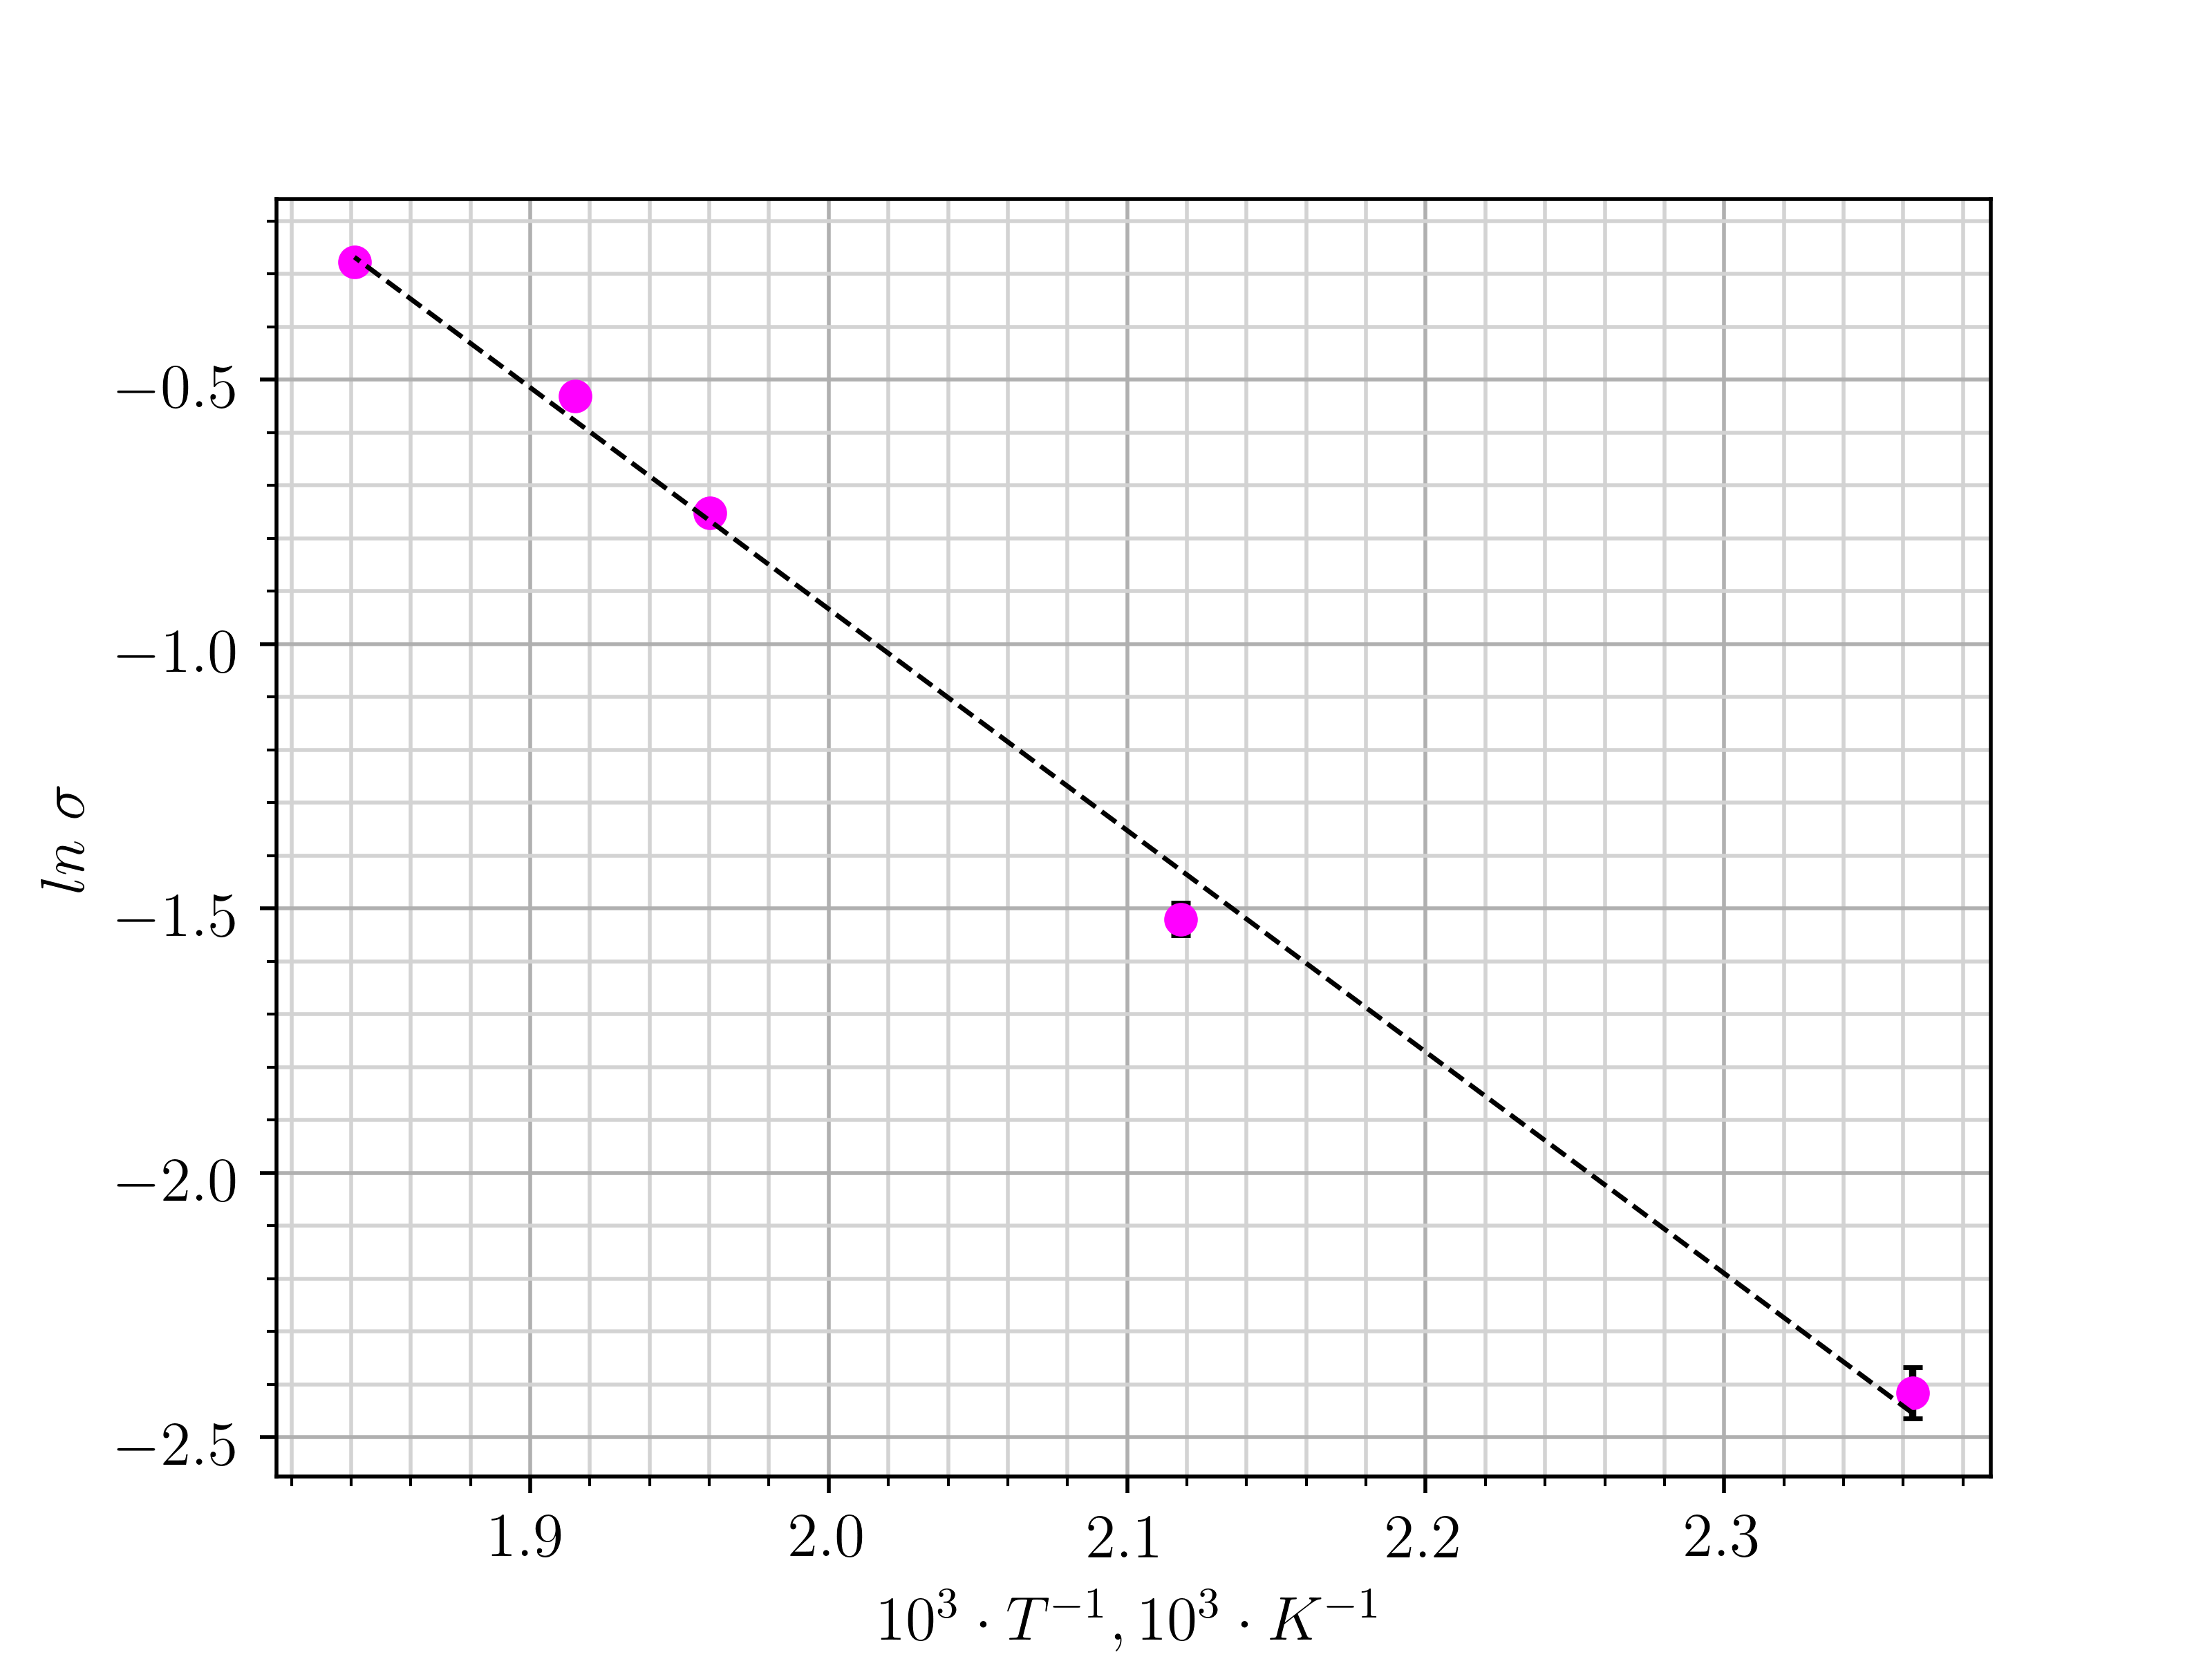
\includegraphics[width = .8\linewidth]{graphs/lns2.png}
	\caption{}
	\label{fig:exp.2}
\end{figure}

Определили угловой коэффициент наклона кривой в области высоких температур и рассчитали значение $W_g$:
$$\tan(\theta) \approx \py{round(pp[0],2)} \pm 0.5 $$
$$ W_g \approx \py{round(Wg,2)} \pm 0.09\text{ эВ}$$ 

В области истощения примесей (на рис.\ref{fig:exp.1} - область значений от 2.8 до 3.5 по оси $(\frac{10^3}{T})$ )
определили зависимость $\sigma = f(T)$, считая, что $\sigma \approx T^n$. Ее можно найти, взяв на кривой две точки и
воспользовавшись соотношением $\sigma_{I} / \sigma_{2}=\left(T_{I} / T_{2}\right)^{n}$.

% $$\ln \sigma_1 = -4.659, \ln \sigma_2 = -4.644$$
% $$ T_1 = 301.15,T_2 = 305.15 \text{ K} $$
% $$ \ln \sigma_1 - \ln \sigma_2 = n \ln(\frac{T_1}{T_2})$$
% $$ -4.659+4.644 = n \ln(\frac{301.15}{305.15}) $$
Получаем 
$$ n = \py{round(n,2)} $$

Определили (экстраполяцией по графику) величину $\sigma_c$, соответствующую
электропроводности вещества при $T \to \infty$.
\pyc{sigmainf=round(pp[1],2)}
$$ \ln \sigma_c = \ln \sigma (T \to \infty) = \py{sigmainf}$$
$$\sigma_c = e^{\py{sigmainf}}  = \py{round(e**sigmainf,2)} \text{ Ом$^{-1}$см$^{-1}$}$$


\end{document}
